\section{Aktuelle Situation und Vergleich der Emulation}
Ein wichtiger Bestandteil in der dynamischen Analyse von Apps ist die Möglichkeit Applikationen  in einer emulierten Umgebung auszuführen. Im Folgenden werden diese Möglichkeiten für die iOS, Windows-Phone und Android getestet.
 
	\subsection{iOS}
	Im Folgenden wurde speziell die der in XCode enthaltene, offizielle IPhone-Simulator in seiner Funktionsweise untersucht.
	
			\subsubsection{Emulation}\label{ref:emulation}
			Die Emulation von iOS-Geräten ist derzeit mit der Verwendung von XCode möglich. XCode wiederum ist nur unter Mac OS X erhältlich. Da Max OS X laut EULA nur auf "`Apple-branded computers"' verwendet werden darf \cite{AppleEULA}, ist die Simulation von iOS-Geräten nur unter Apple-Hardware möglich. Nach der Installation über den in Mac OSX enthaltenen App-Store kann ein virtualisiertes IPhone über die Schritte XCode $\rightarrow$ Open Developer Tools $\rightarrow$ Simulator oder über 
\begin{lstlisting}
/Applications/Xcode.app/Contents/Developer/Applications/Simulator.app
\end{lstlisting}			
gestartet werden.\\
			
		\subsubsection{Debugging}
Als Debugger unter \textit{Mac OS X} hat sich \textit{LLDB} etabliert und stellt das Pendant zu GDB unter Linux dar. \textit{LLDB} ist kostenlos verfügbar, Open-Source und steht unter der University of Illinois/NCSA Open Source License\footnote{\url{https://opensource.org/licenses/UoI-NCSA.php}}, welche die Vervielfältigung und Veränderung des Quellcodes unter unter Hinweis auf \textit{LLVM} erlaubt.\\

\textit{LLDB} sollte auf jedem \textit{Mac OS X} System mit \textit{XCode} automatisch installiert sein und lässt sich im Terminal über das Kommando
\begin{lstlisting}
lldb
\end{lstlisting} aufrufen. Eine Gegenüberstellung von GDB-Kommandos zu LLDB steht auf der LLDB-Webseite\footnote{\url{http://lldb.llvm.org/lldb-gdb.html}} zur Verfügung.\\

 Kompiliert man eine Applikation in XCode, wird diese in einem emulierten IPhone gestartet und direkt ein Fenster LLDB hergestellt. Die ausgeführte Applikation ist in LLDB automatisch ausgewählt.\\

\begin{figure}[htbp]
	\centering
	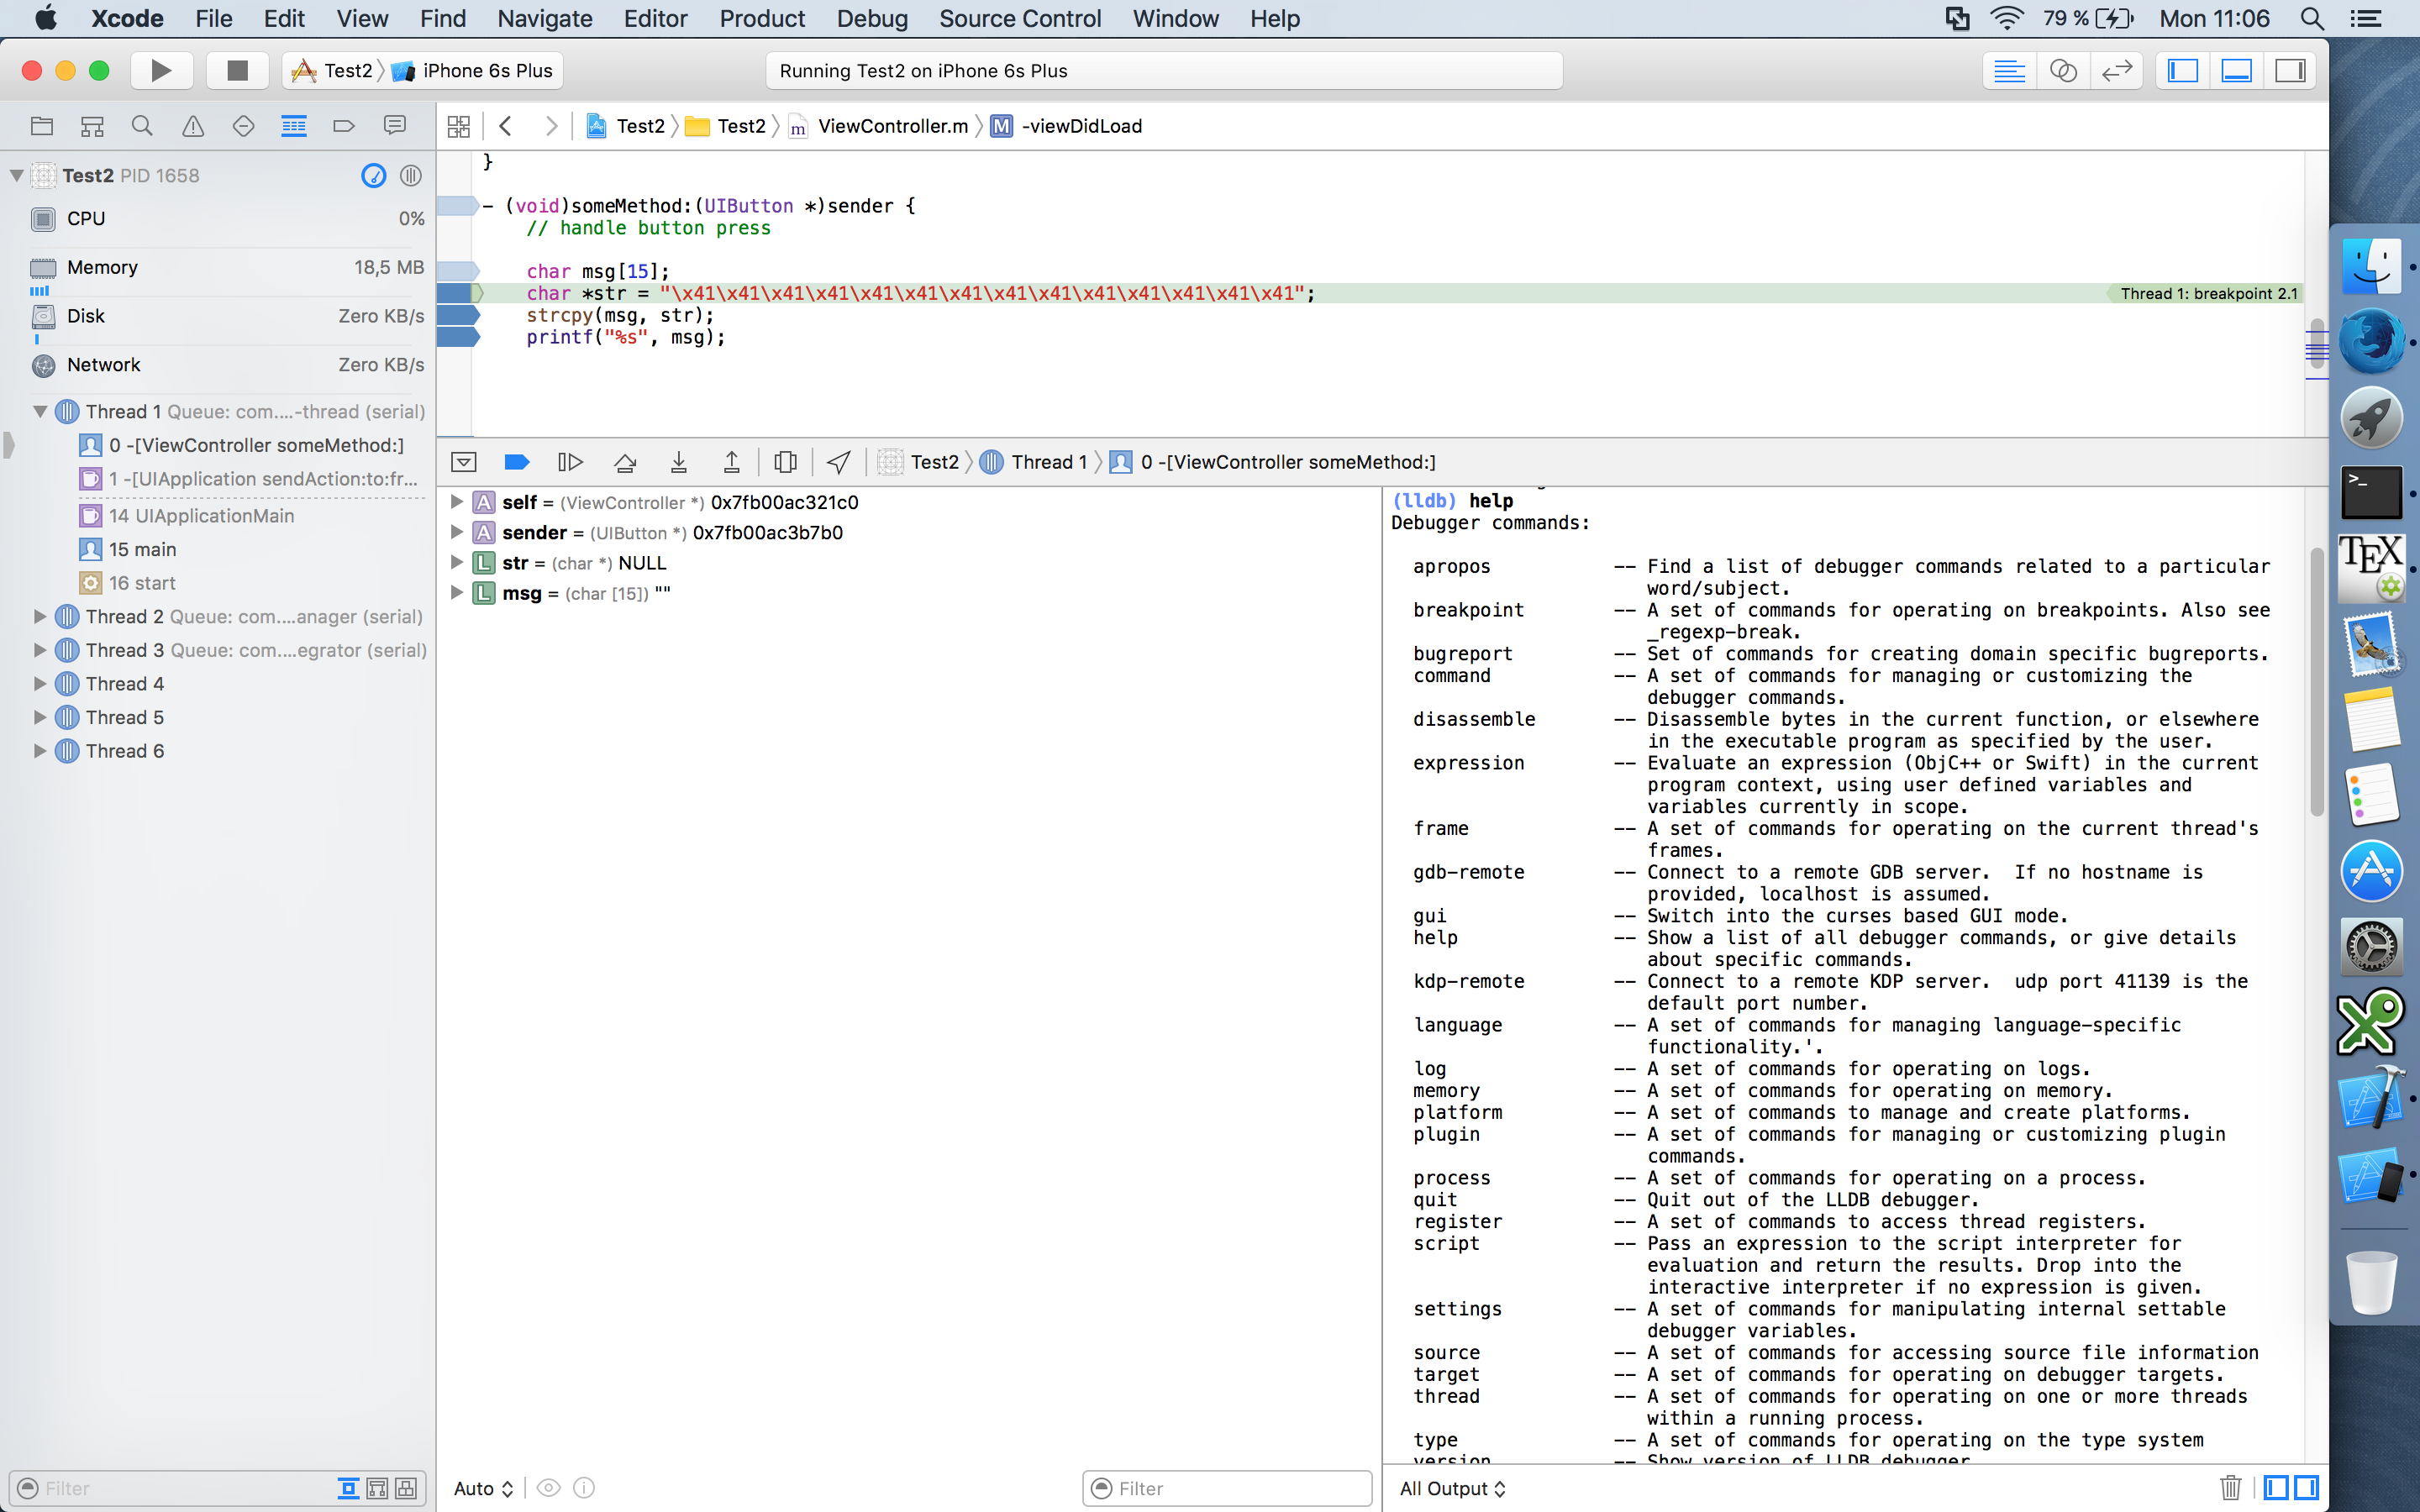
\includegraphics[width=\textwidth]{bilder/pentest_mobile_anwendungen/vergleich_aktuelle_situation/20160627_XCode-LLDB.png}
	\caption{LLDB in XCode}
	\label{fig:LLDBinXCode}
\end{figure}
Ein Ziel dieser Arbeit ist jedoch das Automatisieren von Analysen, weshalb das Ausführen der grafischen Oberfläche nicht optimal ist.\\

Leider ist nicht erkennbar, wie \textit{LLDB} und das emulierte IPhone eine Verbindung herstellen. Eine Auflistung der offen Sockets auf dem System legt jedoch nahe, dass auf dem IPhone das Programm \textit{debugserver} gestartet wird, welches Remote-Debugging mit \textit{LLDB} erlaubt. Es bleibt herauszufinden, wie die Debugging-Session auf dem simulierten IPhone ohne XCode hergestellt werden kann.\\

\begin{figure}[htbp]
	\centering
	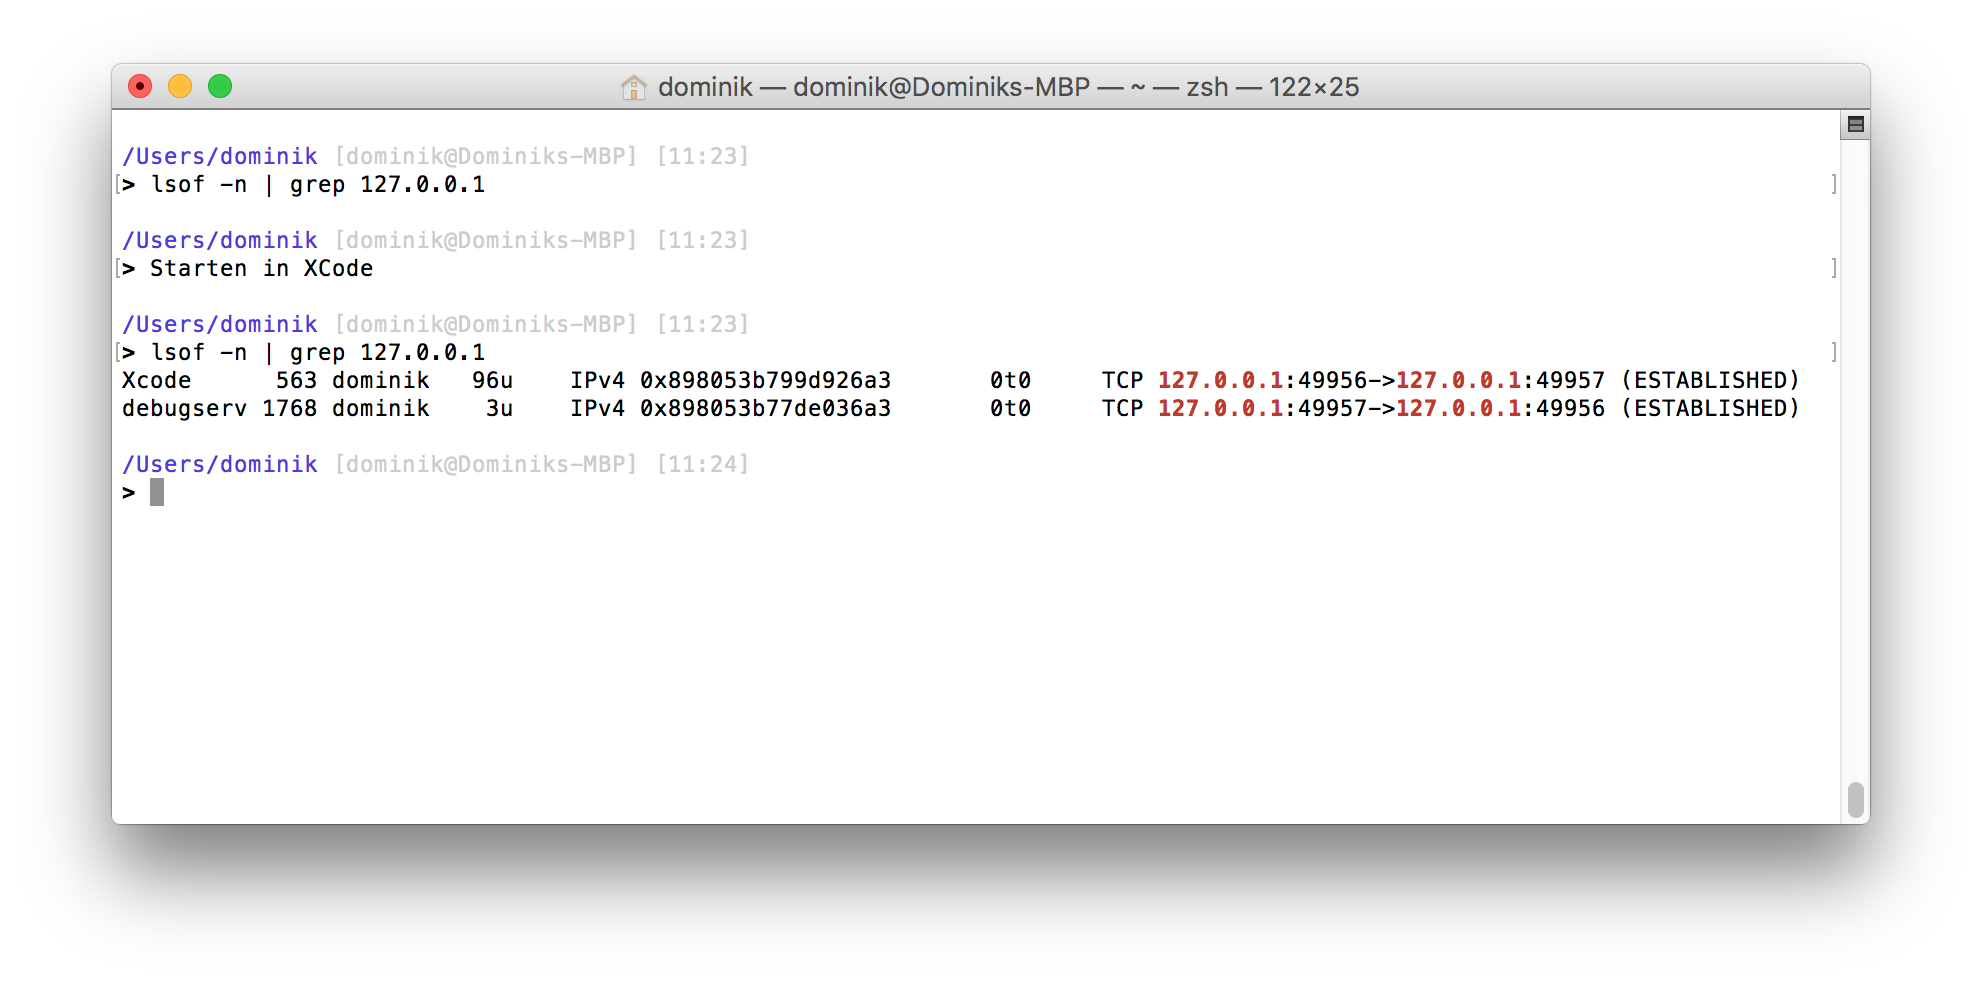
\includegraphics[width=\textwidth]{bilder/pentest_mobile_anwendungen/vergleich_aktuelle_situation/20160627_lsof_XCode_running.png}
	\caption{Vergleich der offenen Pipes vor und nach der Ausführung der Applikation in XCode}
	\label{fig:LSOFLLDB}
\end{figure}

Nach einem Artikel von Apple\footnote{\url{https://developer.apple.com/library/ios/documentation/IDEs/Conceptual/gdb_to_lldb_transition_guide/document/lldb-terminal-workflow-tutorial.html}}, ist es möglich, mit  LLDB eine App auch als "`Standalone Debugger"', also ohne XCode, zu verwenden. Dies ist in Abbildung \ref{fig:LLDBStandaloneDebugger} aufgezeigt.\\

\begin{figure}[htbp]
	\centering
	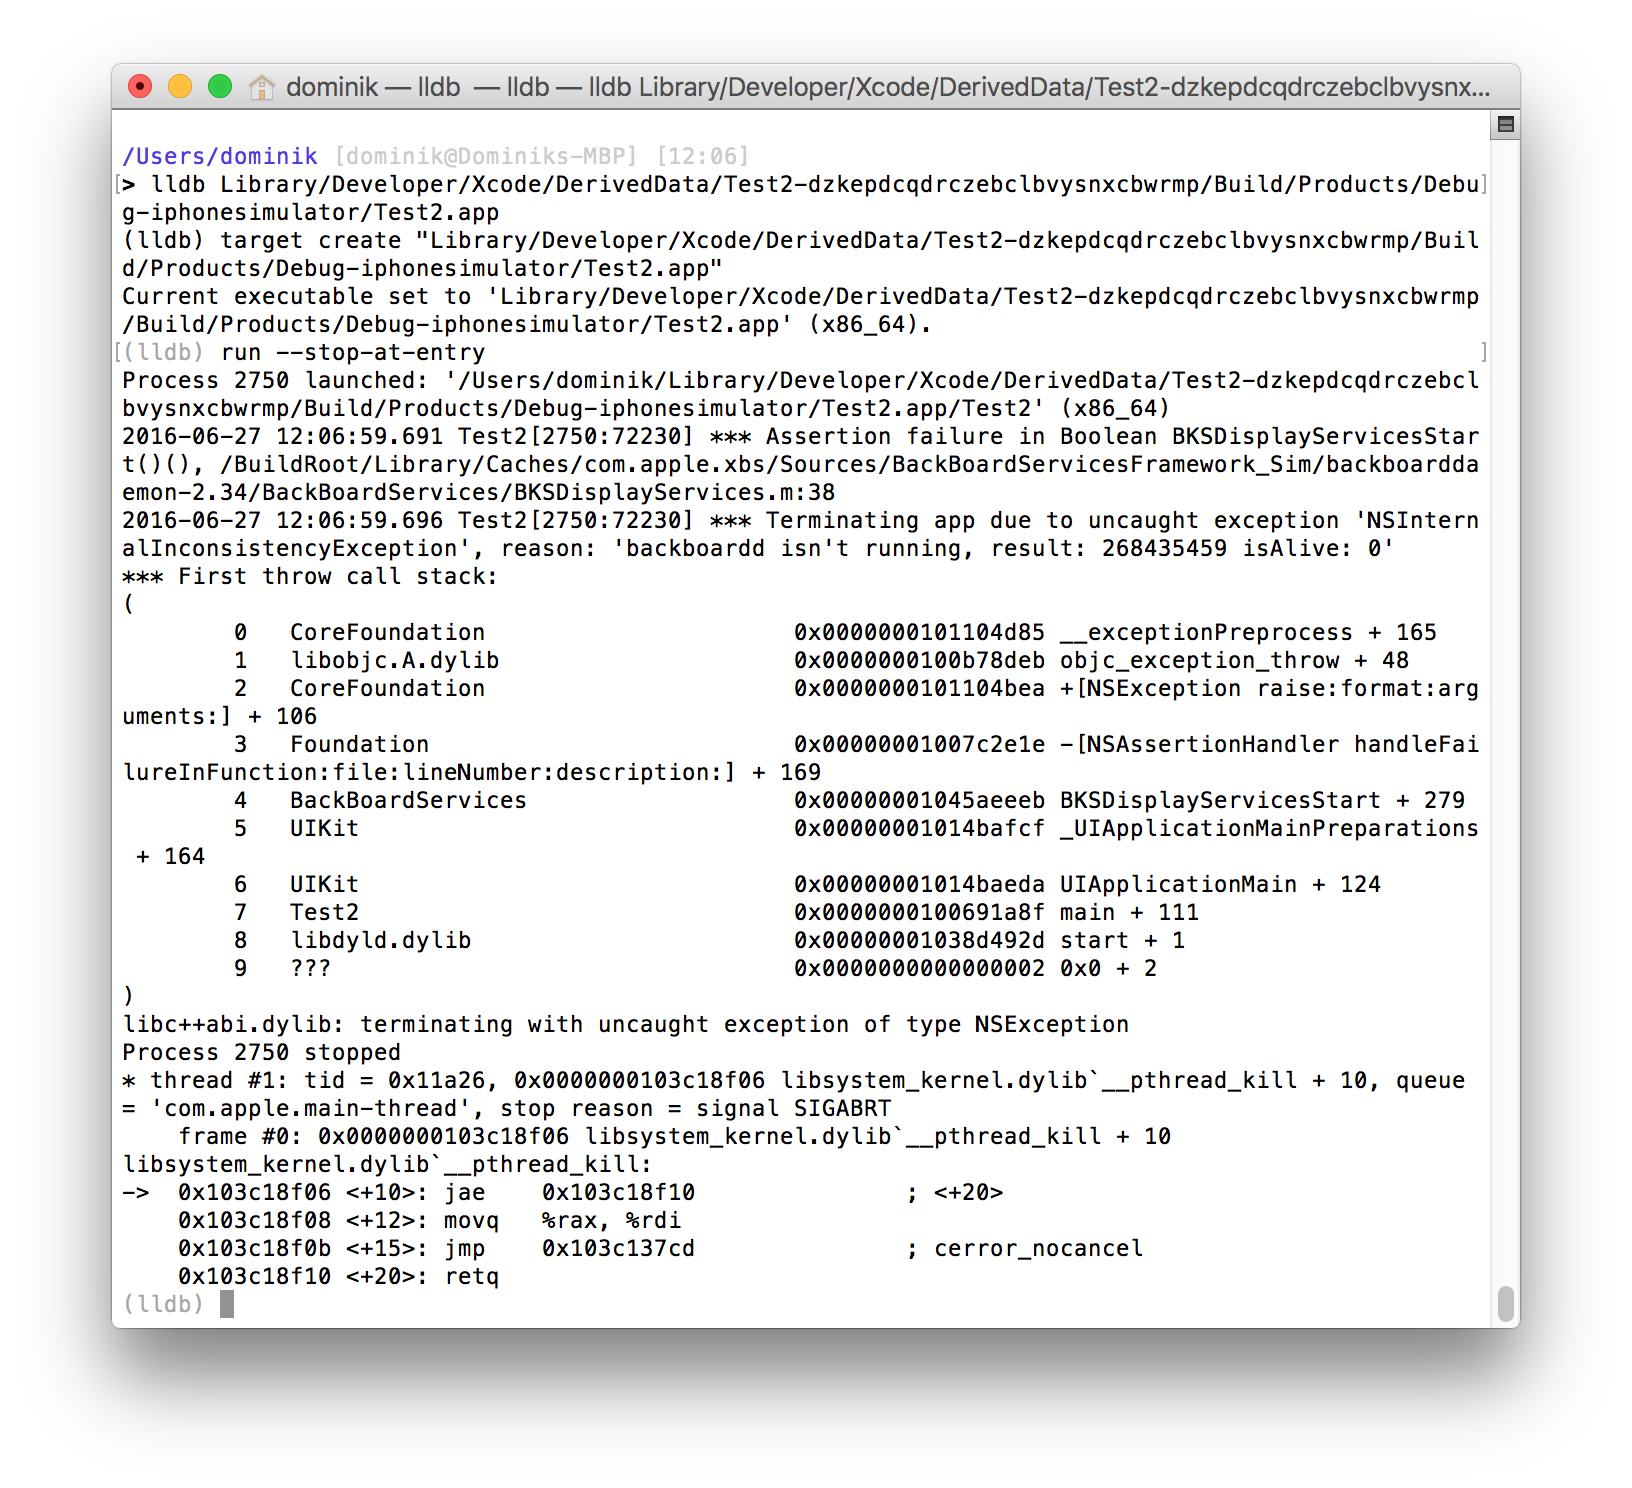
\includegraphics[width=\textwidth]{bilder/pentest_mobile_anwendungen/vergleich_aktuelle_situation/20160627_LLDB-Standalone-Debugger.png}
	\caption{LLDB als Standalone Debugger}
	\label{fig:LLDBStandaloneDebugger}
\end{figure}

Um zu verifizieren, dass die App auf einem simulierten IPhone ausgeführt wird, können entweder die geöffneten Prozesse (siehe Abbildung \ref{fig:LLDB-creating-IPhone-VM}) oder die geladenen Bibliotheken der Programme (siehe Abbildung \ref{fig:VergleichLLDBImages}) verglichen werden.\\

\begin{figure}[htbp]
	\centering
	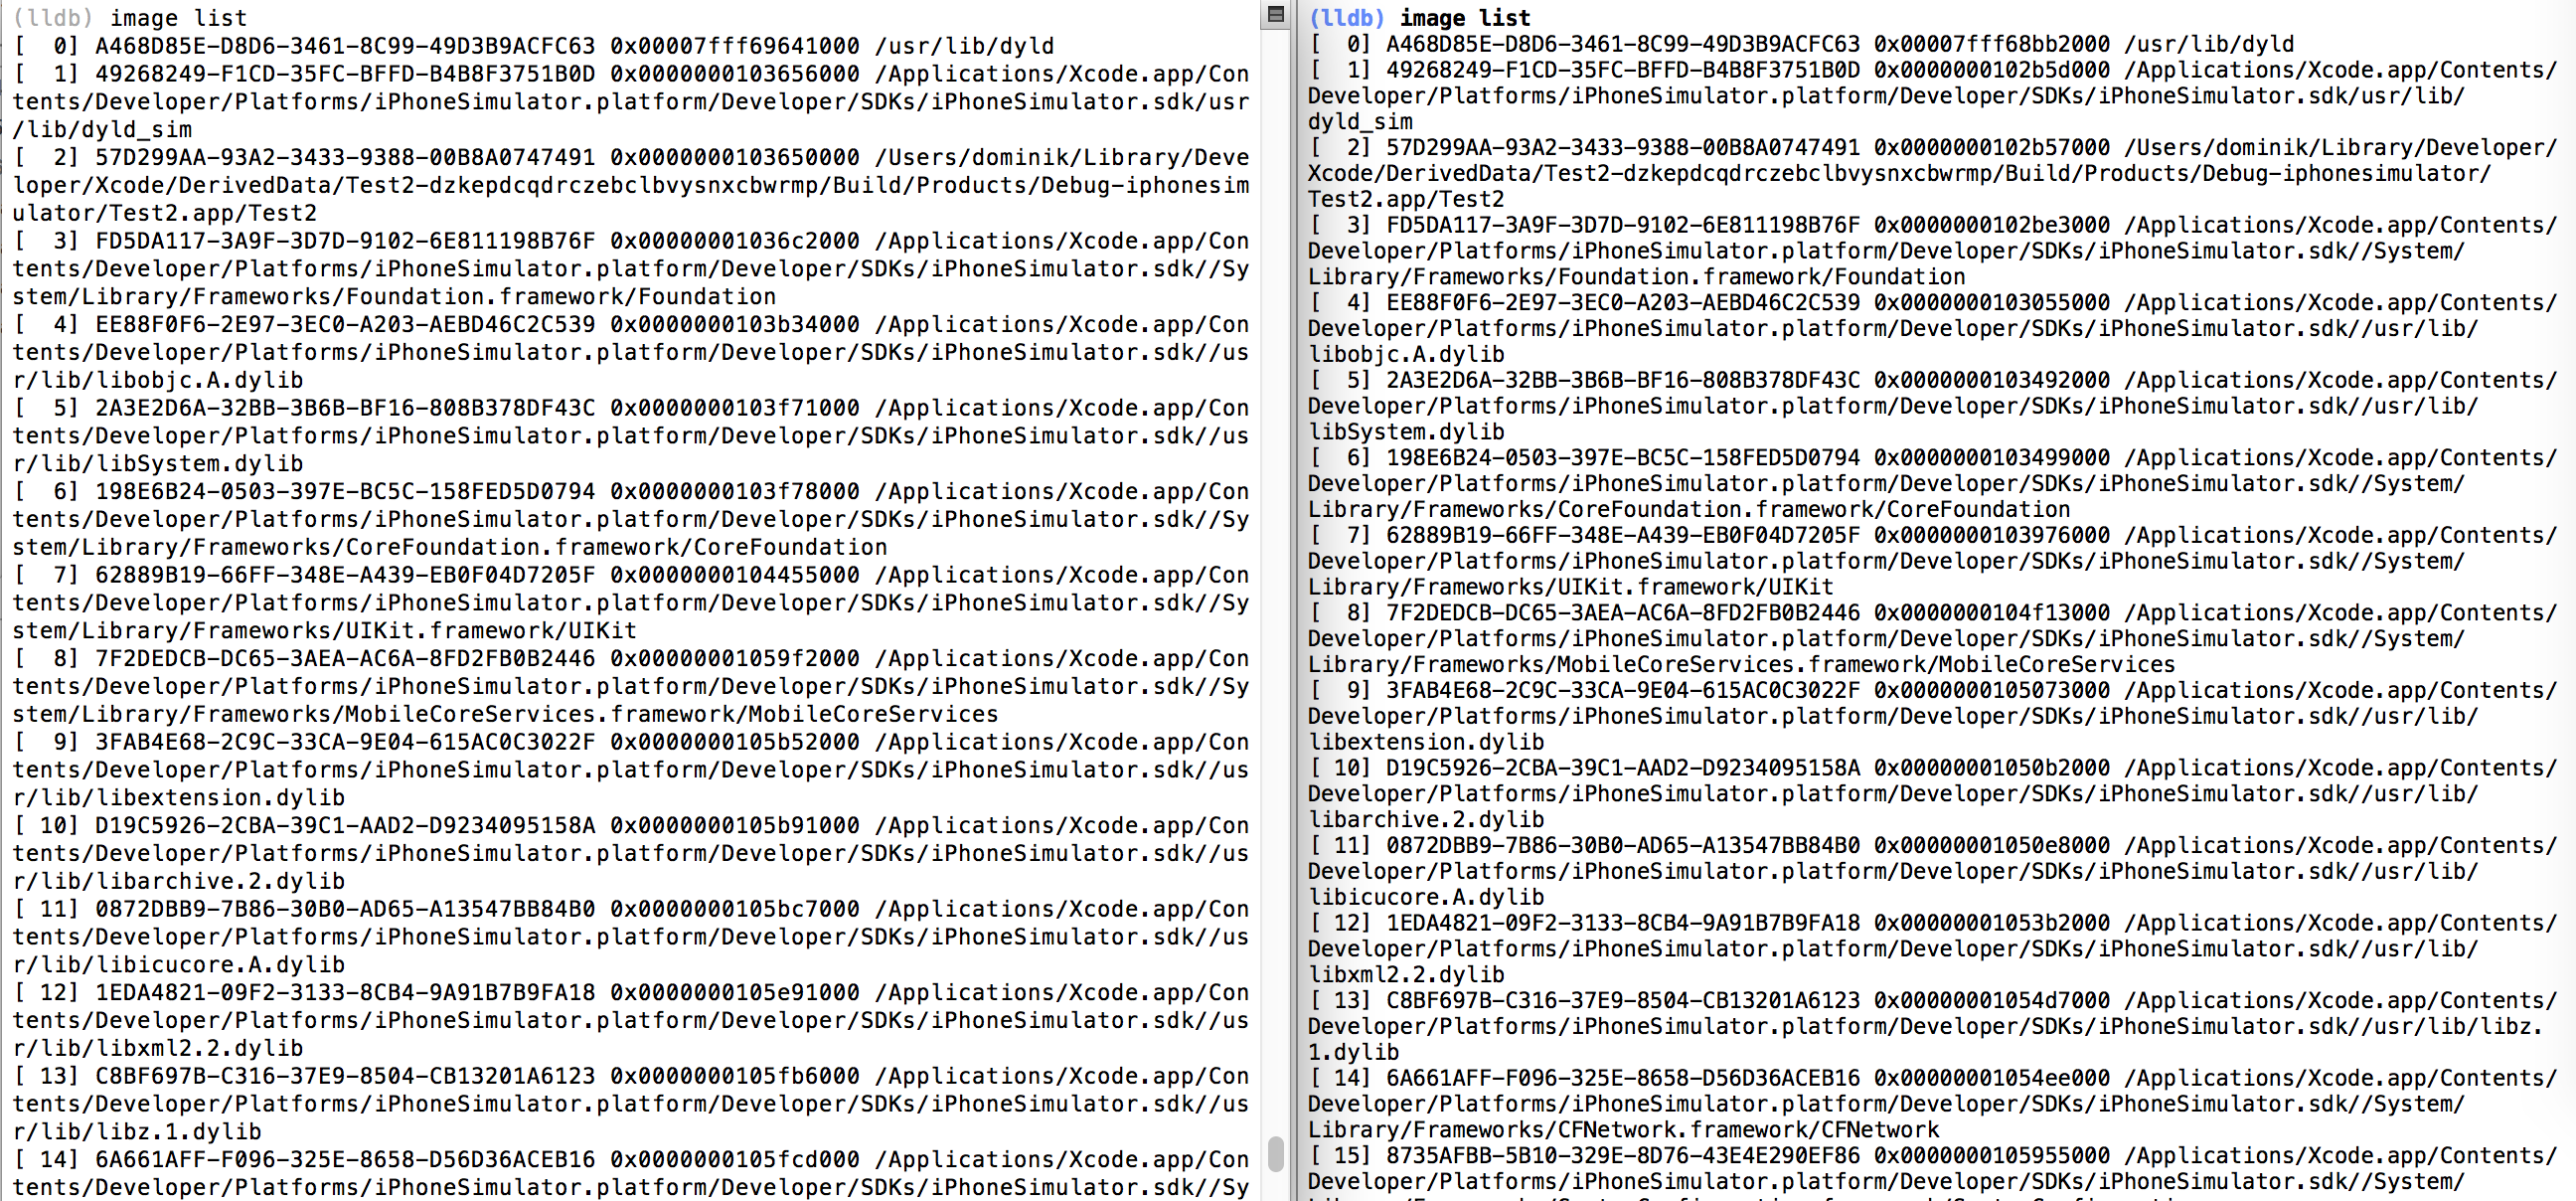
\includegraphics[width=\textwidth]{bilder/pentest_mobile_anwendungen/vergleich_aktuelle_situation/20160627_LLDB-image-list.png}
	\caption{Vergleich der geladenen Bibliotheken}
	\label{fig:VergleichLLDBImages}
\end{figure}

Bei Methoden zeigen, dass die App auf dem simulierten IPhone gestartet wird. Bei den Prozesse ist zu beobachten, dass vor Start von LLDB nur der Hintergrund-Service ausgeführt wurde. Nach dem Start von LLDB dagegen läuft der gesamte Simulator.\\

Auch der Vergleich der geladenen Bibliotheken legt nahe, dass die LLDB Standalone und XCode in der gleichen Umgebung ausgeführt werden. Die Adressen im RAM variieren aufgrund von ASLR zwar, aber es werden die selben Bibliotheken verwendet (am Pfad zu erkennen). Dies ist in Grafik \ref{fig:VergleichLLDBImages} dargestellt.\\

\begin{figure}[htbp]
\lstinputlisting[caption={Gestartete Prozesse nach LLDB Aufruf},lastline=16]{logs/20160627_LLDB-creating-IPhone-VM.txt}
\label{fig:LLDB-creating-IPhone-VM}
\end{figure}

\subsubsection{Architektur}
Auffällig ist, dass der Simulator nicht die CPU-Architektur eines IPhones simuliert, sondern den Code auf dem x86-Prozessor des Mac-Books ausführt. Dies hat den Nachteil, dass Apps aus dem Apple-App-Store, welche für ARM-Prozessoren kompiliert sind, nicht auf dem Simulator ausgeführt werden können. Lediglich Apps, welche für den Simulator in XCode kompiliert wurden, können im Simulator ausgeführt werden. Dadurch ist eine Analyse von Apps ohne Quellcode-Zugriff nicht möglich.

\subsubsection{Sicherheits-Aspekte}
Bei Analyse von iOS-Apps wurden zwei mögliche Sicherheits-Lücken testweise in eine App implementiert. Die Lücken sind "`unsichere Funktionen"', welche eine eventuelle Memory Corruption mit sich ziehen, und Verbindungen ohne TLS-Absicherung.

\paragraph{Unsicher Funktionen}
In Objective C für iOS-Apps sind Funktionen, welche für Memory Corruption-Schwachstellen bekannt sind, leider noch vorhanden.\\

So führt folgendes Code-Segment zwar zum Absturz der App, aber könnte bei einer dynamischen Eingabe des zu kopierenden Strings durchaus eine echte Schwachstelle einführen.
\begin{lstlisting}
char msg[15];
char *str = "\x41\x41\x41\x41\x41\x41\x41\x41\x41\x41\x41\x41\x41\x41\x42";
strcpy(msg, str);
\end{lstlisting}

Dies ist auch in der Apple-Online-Dokumentation beschrieben\footnote{\url{https://developer.apple.com/library/content/documentation/Security/Conceptual/SecureCodingGuide/Articles/BufferOverflows.html}}.

\paragraph{Ungesicherte Verbindungen}\label{ref:inseccon}$ $\\
Ein Sicherheits-Feature ab iOS 9.0 ist der Umgang von iOS mit Netzwerk-Verbindungen. So können ohne erweitere Konfiguration keine Verbindungen aufgebaut werden, welche nicht dem RFC-Standard 2818\footnote{\url{https://tools.ietf.org/html/rfc2818}} folgen. So wird folgender Aufruf einer HTTP-Seite
\begin{lstlisting}
NSURL *url = [NSURL URLWithString:@"http://api.ipify.org"];
    NSData *data = [NSData dataWithContentsOfURL:url];
    NSString *ret = [[NSString alloc] initWithData:data encoding:NSUTF8StringEncoding];
    NSLog(@"ret=%@", ret);
\end{lstlisting} blockiert und folgende Fehlermeldung generiert:
\begin{lstlisting}
2016-06-28 08:42:56.518 Test2[4789:140270] App Transport Security has blocked a cleartext HTTP (http://) resource load since it is insecure. Temporary exceptions can be configured via your app's Info.plist file.
\end{lstlisting}

Sollten unsicher Verbindungen benötigt werden, muss ein entsprechender Eintrag in der "`Info.plist"' angelegt werden. Dieser Eintrag muss sehr genau auf die App angepasst werden, da zum Beispiel die Domains festgelegt werden müssen. Ein Eintrag muss laut Apple\cite{AppleNSAppTransportSecurity} folgenden Inhalt haben:
\begin{lstlisting}
NSAppTransportSecurity : Dictionary {
    NSAllowsArbitraryLoads : Boolean
    NSAllowsArbitraryLoadsForMedia : Boolean
    NSAllowsArbitraryLoadsInWebContent : Boolean
    NSAllowsLocalNetworking : Boolean
    NSExceptionDomains : Dictionary {
        <domain-name-string> : Dictionary {
            NSIncludesSubdomains : Boolean
            NSExceptionAllowsInsecureHTTPLoads : Boolean
            NSExceptionMinimumTLSVersion : String
            NSExceptionRequiresForwardSecrecy : Boolean   // Default value is YES
            NSRequiresCertificateTransparency : Boolean
        }
    }
}
\end{lstlisting}

Eine Überprüfung auf solche Ausnahmen kann dem Abschnitt \ref{ref:WeitMobSFErkennungVonUngesichertenVerbindungen} entnommen werden.

		\subsection{Windows-Phone}
			\subsubsection{Emulation vs. Hardware}
			VS
			\subsubsection{Debugging}
			VS
			
		\subsection{Android}
			Android ist ein Ursprünglich 2003 von der Android, Inc. entwickeltes mobiles Betriebssystem. 2005 wurde es durch Google übernommen und wird seit dem weiterentwickelt. 2015 liegt es bei einem Marktanteil von TODO \%. Aufgrund der Quelloffenheit des Systems wird von vielen Herstellern auf verschiedensten Plattformen genutzt. Jedoch bringt die weitführende Fragmentierung des Betriebssystems auch Nachteile mit sich. So sind in 2015 nur TODO \% der Android-Devices auf einer aktuellen Version.\cite{Drake2014}
			
			\subsubsection{Android-Studio und SDK}
			Das Android-Studio ist eine umfassende IDE. Sie ermöglicht unter anderem das schnelle Entwickeln und Testen von Apps, sowie die Emulation von beliebigen Android-Versionen. Außerdem ist Android Studio kostenlos, Open-Source und für Linux, Mac und Windows erhältlich. Die aktuelle Version kann unter \url{http://developer.android.com/sdk/index.html} heruntergeladen werden. Die Installation unter Linux ist vergleichsweise einfach, da nur ein Archiv über das Kommando 
\begin{lstlisting}
unzip android-studio-ide-143.2739321-linux.zip
\end{lstlisting}
entpackt werden muss. Für alle anderen Betriebssysteme werden entsprechende Installationsroutinen zur Verfügung gestellt. Anschließend kann die IDE über die Datei "`bin/studio.sh"' gestartet werden. Neben dem Android-Studio gibt es noch das Android SDK, welches über die gleiche URL heruntergeladen werde kann. Es enthält wichtige Kommandozeilen-Tools wie \textit{adb}, \textit{fastboot} oder \textit{logcat}, auf welche im weiteren Verlauf noch detailliert eingegangen wird.

			\subsubsection{Compatibility Testing Suite}
			\cite{Drake2014} Seite 18
			
			\subsubsection{Emulation vs. Hardware}
			Android SDK; AVD
			Im Gegensatz zum iOS-Simulator hat AVD die Möglichkeit CPU wie auch GPU eines Handys zu emulieren. Dabei besteht die Auswahl zwischen verschiedenen Architekturen, wie Intel x86 oder ARM. Zudem gibt es viele andere Möglichkeiten zur Konfiguration der einzelnen Maschinen, wie in Grafik \ref{fig:VergleichAVDConfig} zu sehen ist. Daher hat Android den Vorteil, dass gerade tiefgreifende Analysen aufgrund der Emulation der Architektur näher an der echten Hardware sind als bei iOS.
			
			\begin{figure}[htbp]
				\centering
				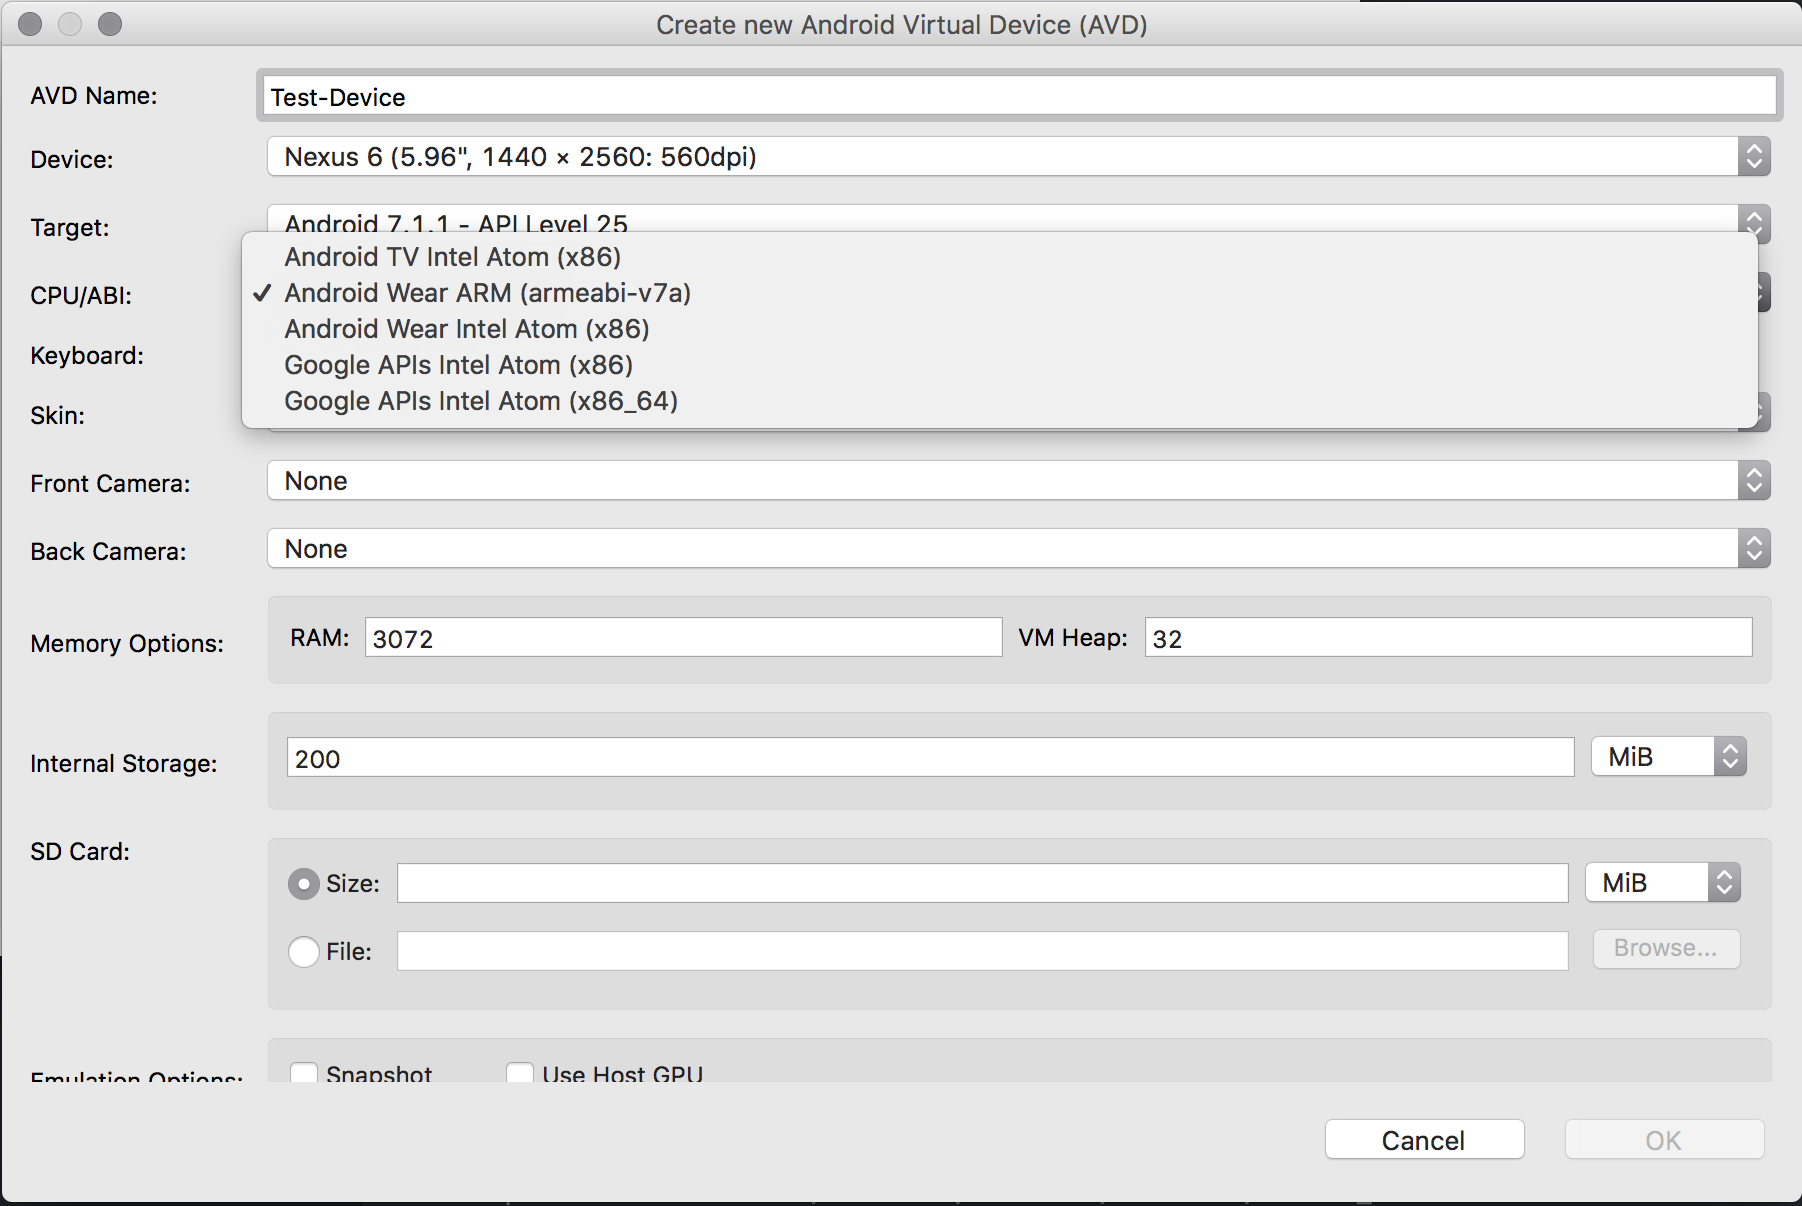
\includegraphics[width=\textwidth]{bilder/pentest_mobile_anwendungen/vergleich_aktuelle_situation/20170215_AVD-Config-Screen.png}
				\caption{Der Konfigurations-Bildschirm des AVD-Managers}
				\label{fig:VergleichAVDConfig}
			\end{figure}
			
			TODO: Android-Hackers Handbook
			
			\subsubsection{Debugging}	
			
			Android Debug Bridge\cite{androidDebugBridge}
			
			\subsubsection{Logcat}	
			Android Debug Bridge\cite{androidDebugBridge}